\documentclass[11pt]{article}
\usepackage[margin=1in]{geometry}
\usepackage{biblatex}
\bibliography{main} 
\addbibresource{main.bib}
\usepackage{amsmath}
\usepackage{listings}
\usepackage{graphicx}
\usepackage{subfig}
\usepackage{caption}
\usepackage{float}
\usepackage{todonotes}
\usepackage[export]{adjustbox}
\usepackage{wrapfig}
\usepackage{sidecap}

\title{Machine Learning Review}
\author{Francesco Saverio Zuppichini}
\begin{document}
\maketitle
The aim of this report is to summarise the topics threaded in my Machine Learning class at USI.
\section{History of Machine Learning}
\todo[inline]{Write something about the history of ML}

\section{Gradient Descend}
The gradient descend is an iterative optimisation algorithm that follows the direction of the negative gradient in order to minimised an objective function. It can be effectively used as Learning Algorithm because it reduces the error function, Equation \ref{eq: MSE_perceptron}, and adjusts the weights properly. Equation \ref{eq: GD} shows the generic update rule.
\begin{equation}
\label{eq: gradient_descent}
	w_{k + 1} = w_k - \eta \nabla E(w_k)
\end{equation}
Where $\eta$ is the step size, also called \textbf{learning rate} in Machine Learning. This parameter influences the behaviour of gradient descent, a small number can lead to local minimum, while a bigger learning rate could "over-shoot" and decreasing the converge ration. Later in this project you will see how a wrong $\eta$ can strongly change the output of a Neural Network.

For this reasons, numerous improvements have been proposed to avoid local minima and increase its convergence ration, some of them are: Conjugate Gradient and Momentum.
\section{Perceptron}
\section{Definition}
The \textbf{Perceptron} is binary  \textbf{linear classifier} algorithm used in \textbf{supervised learning}. It can be seen as the most basic form of Neural Network. Equation \ref{eq: perceptron} defines the its output.
\begin{equation}
f(x) \left \{ 
 \begin{tabular}{lcc}
  1 \quad \text{if} w \cdot x + b \ge  0 & & \\ 
  0 \quad \text{otherwise} &  & 
  \end{tabular}	
  \label{eq: perceptron}
\end{equation}
Given a training set $D = \{ (x_1,t_1}, ... , (x_n,t_i) \}$, $x_i \in X$ and $t_i \in Y$ denotes the input vector and the target vector respectively. We express $y = f(x)$ as the output of the algorithm, $w$ the weight and $b$ the bias. At each iteration the error is calculated using the Mean Square Error, defined in equation \ref{eq: MSE_perceptron}
\begin{equation}
\label{eq: MSE_perceptron}
	E(w) = \frac{1}{N}\sum_{i = 1}^N(\underbrace{y(x_i,w_i)}_{\text{predicted}} - \underbrace{t_i}_{\text{actual}})^2)
\end{equation}
The algorithm uses stochastic \textbf{Gradient Descent} in order to update the weight at each iteration using the formula defined in Equation \ref{eq: gradient_descent}.
 
\begin{equation}
	\frac{\partial E}{\partial w_k} = y - t
\end{equation}
\todo[inline]{Decide if use \nabla or partial or booth}
\section{Neural Network}
A \textbf{Neural Network} is a universal function approximation. Basically it is a big chain function composed by layer of $n$ non-linear perceptron. In its simplest representation, an FeedForward Neural Network, it is composed by a \textbf{input layer}, an \textbf{hidden layer} and an \textbf{output layer}. The size of the hidden layer is usually refers as the \textbf{deepth} of the network.
\subsubsection{Forward pass}
In order to get the prediction out of our network we need to calculate the compute the activation at each layer $l$.
Equation \ref{eq:forward_pass} shows the activation $a$ of layer $l$ for the $j$-th neuron on that layer.

\begin{equation}
\label{eq:forward_pass}
a^l_j = \sigma(\sum_k w^l_{jk}a^{l-1}_k + b^l_j)
\end{equation}

Where $w^l_{jk}$ is the connection from neuron $k$ in the $l-1$ layer to $j$, $a^{l-1}$ is the activation of the previous layer and $b^l_j$ is the bias of $j$-th neuron in the $l$ layer. With this in mind, we can rewrite \ref{eq:forward_pass_vectorized} in a efficient vectorised form
\begin{equation}
\label{eq:forward_pass_vectorized}
a^l = \sigma(W^la^{l-1} + b^l)
\end{equation}

\subsubsection{Delta rules}
In a Neural Network the weights are iteratively changed in order to decrease the cost function, called $E$. We want to find out how much they should be updated, in order to do so we need the output error at each layer. Equation \ref{eq:deltaRule_1} defines $\delta^l_j$ as the output error of neuron $j$ in layer $l$
\begin{equation}
	\delta^l_j = \frac{\partial E}{\partial z^l_j}
	\label{eq: deltaRule_1}
\end{equation}
Strictly speaking, $\delta^l_j$, is how much the error function changes by changing the weighted input on that layer. Applying the chain rule, Equation \ref{eq: deltaRule_1} becomes:
\begin{equation}
\delta^l_j = \frac{\partial E}{\partial a^l_j} \frac{\partial a^l_j}{\partial z^l_j}
\label{eq:deltaRule_2}
\end{equation}
By knowing that $a^l_j = \sigma(z^l_j)$, Equation \ref{eq:deltaRule_2} can be expressed as
\begin{equation}
\delta^l_j = \frac{\partial E}{\partial a^l_j} \sigma'(z^l_j)
\label{eq:deltaRule}	
\end{equation}
\subsubsection{Back Propagation}
The \textbf{Back Propagation} algorithm defines an efficient and interactive method to calculate the gradient at each layer. We want to compute $\frac{\partial E}{\partial w^l_{jk}}$. We can applying the delta rule: 
\begin{equation}
\frac{\partial E}{\partial w^l_{jk}} = \frac{\partial E}{\partial z^l_j}\frac{\partial z^l_j}{\partial w^l_{jk}} =	
\frac{\partial E}{\partial a^l_j}\frac{\partial a^l_j}{\partial z^l_{j}}
\end{equation}
After some calculation, Equation \ref{eq: back_propagation} shows how to calculate the gradient for the weight $w$ of the $l$-th layer for the $j$-th neuron.
\begin{equation}
\frac{\partial E}{\partial w^l_{jk}} = a^{l-1}_k \delta^l_j
\label{eq: back_propagation}
\end{equation}  
\section{Convolutional Neural Network}
\section{Recurrent Neural Network}
\subsection{Definition}
A Recurrent Neural Networks can remember past decision by taking as input not only the current input but also the last time state. For this reason it is said that a RNN has \textbf{memory}. Figure \ref{fig: RNN} shows a classic representation. Usually, a RNN is represented unfolded to highlight the time dependencies. Due to its ability to remember it mostly used in text and speech recognition.
\begin{figure}[h]
\centering
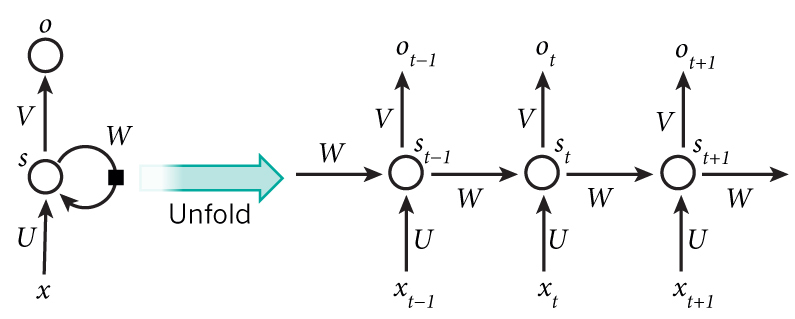
\includegraphics[scale=0.4]{images/rnn}	
\caption{Fold and Unfold representation of a RNN}
\label{fig: RNN}
\end{figure}

Very similar to a feedforward network, Equation \ref{eq: output_rnn} shows the weighted output at layer $j$. The first term on the right-hand is just the feedforward's weighted output, while the second term is the time-dependent term. Matrix $\omega$ is a hidden-state-to-hidden-state matrix. Basically, we are adding previous informations to out new state at time $t$.

\begin{equation}
z[t]^l = (W^la[t]^{l -1}+ b^l_j) + (\omega^l a[t-1]^{l-1})
\label{eq: output_rnn}	
\end{equation}
Equation \ref{eq: activation_rnn} shows the activation of layer $j$ at time $t$.

\begin{equation}
a[t]^l	= \sigma(z[t]^l)
\label{eq: activation_rnn}
\end{equation}


\section{Long Short Term Memory}
\subsection{Definition}
The Long Short Term Memory networks, or just \textbf{LSTM}, are a special type of RNN capable of learning long-term
dependencies. They were introduced by \todo[inline]{metti ref a smitty}. They are composed by LSTM cell, 
Figure \ref{fig: unrolled_LSTM} shows a unrolled representation.
\begin{figure}[h]
\centering
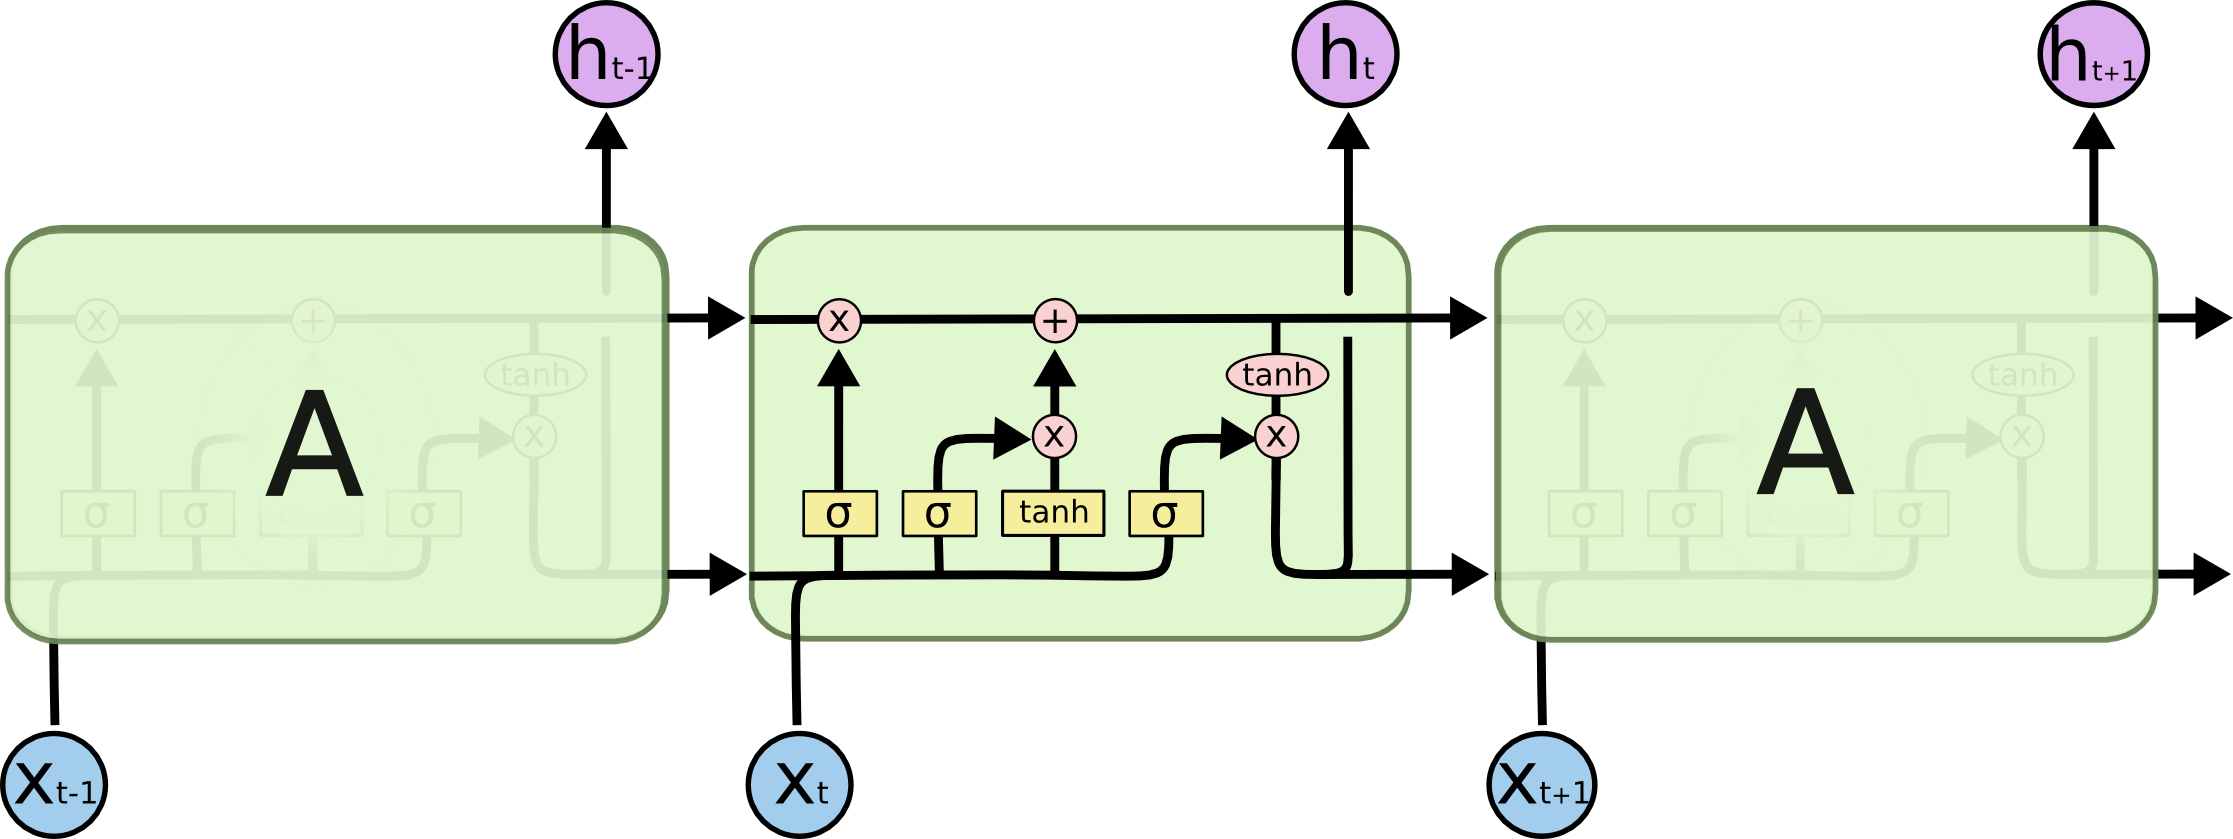
\includegraphics[scale=0.5]{./images/LSTM3-chain.png}	
\caption{An unrolled LSTM}
\label{fig: unrolled_LSTM}
\end{figure}
Each cell is composed by 3 gate: \textbf{forget} gate ($f_t$), \textbf{input} gate $i_t$ and \textbf{output} gate ($o_t$). It takes as 
input the previous output $h_{t - 1}$ and the old cell state $C_{t-1}$, it outputs the next prediction and state, $h_{t}$ and $C_t$. The cell
computes four basic operations:  
% \begin{enumerate}
	% \item
\begin{enumerate}
	\item Forget Gate \\ 
		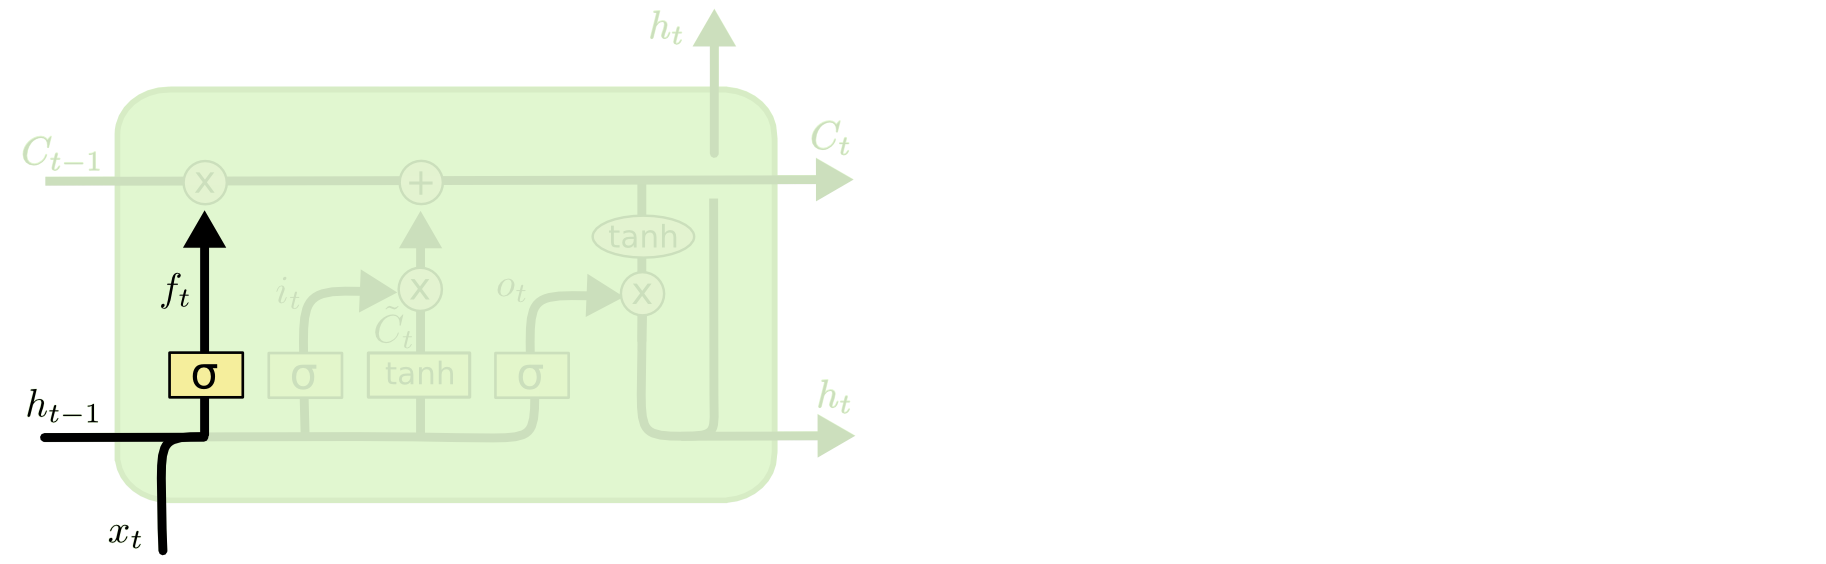
\includegraphics[scale=0.5]{./images/LSTM3-focus-f.png}
\item Input Gate \\
 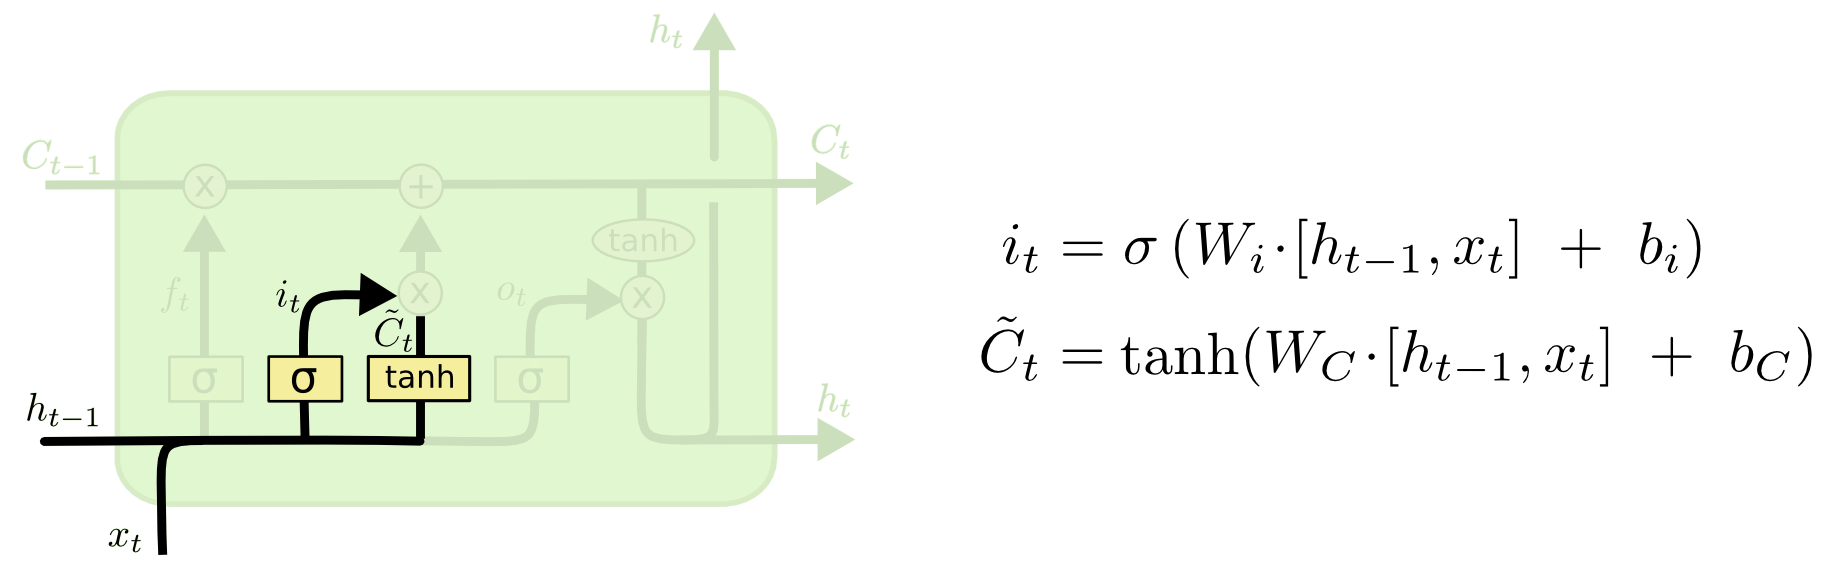
\includegraphics[scale=0.5]{./images/LSTM3-focus-i.png}
\item Update Cell State \\
		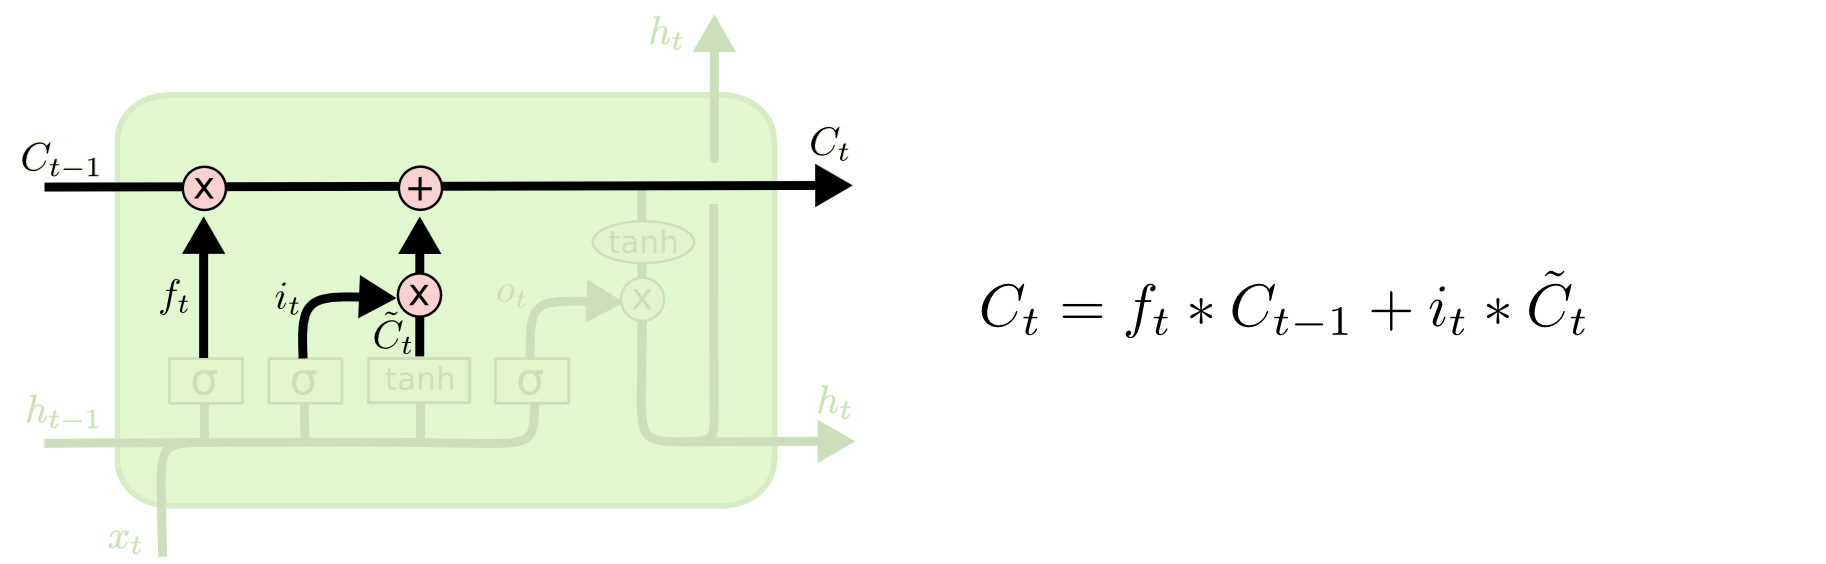
\includegraphics[scale=0.5]{./images/LSTM3-focus-C.png}
\item Output Gate	\\
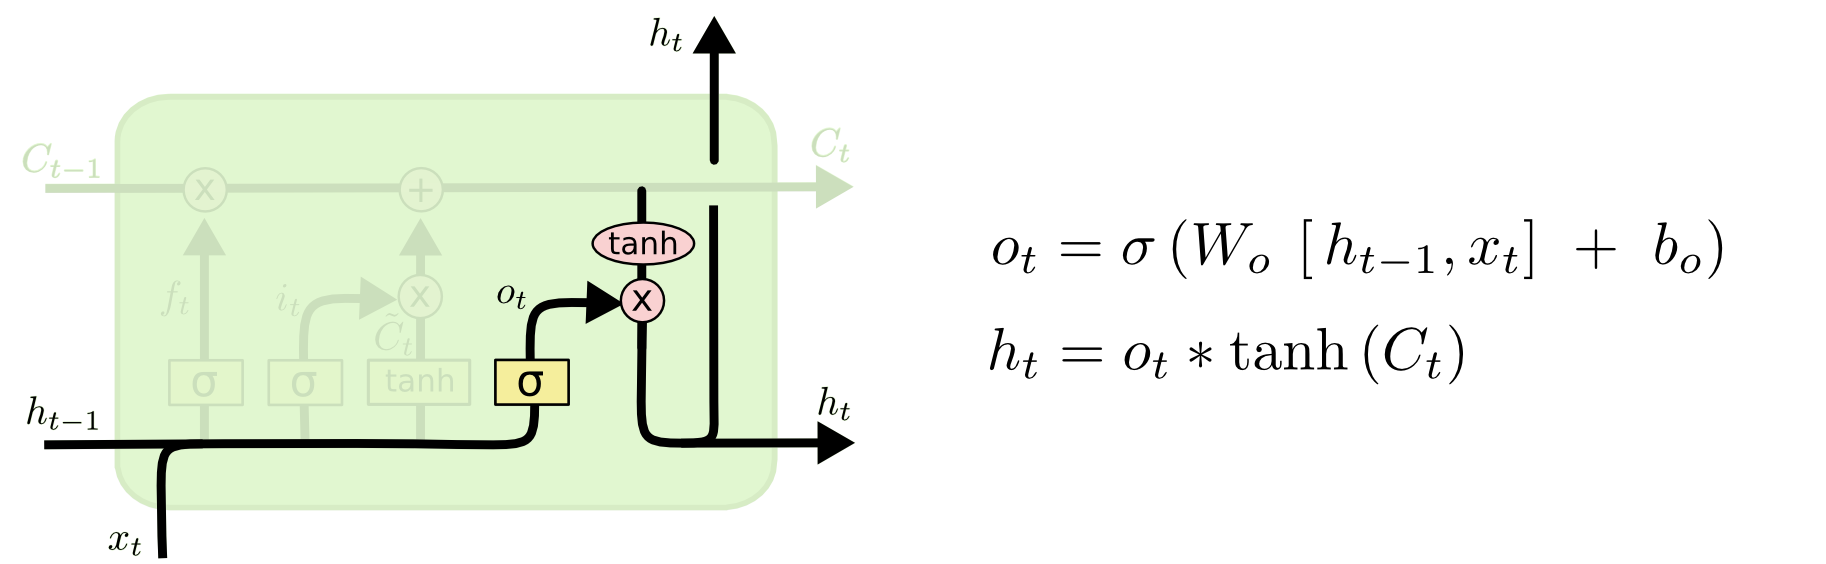
\includegraphics[scale=0.5]{./images/LSTM3-focus-o.png}
\end{enumerate}
	
% \end{enumerate}
\section{Support Vector Machine}
\section{Deep Learning}
\subsection{Training Techniques}
\subsubsection{Mini-batch}
\subsection{Regularisation}
\subsubsection{L1 Regularisation}
\subsubsection{Dropout Regularisation}
\subsection{Activations Functions}
\end{document}
